\chapter{System Description}\label{ch:system-description}

% TODO Write some chapter introduction

% ===============
% MODEL ARCHITECTURE
% ===============

\section{Model Architecture}
 
\begin{figure}[h]
\centering
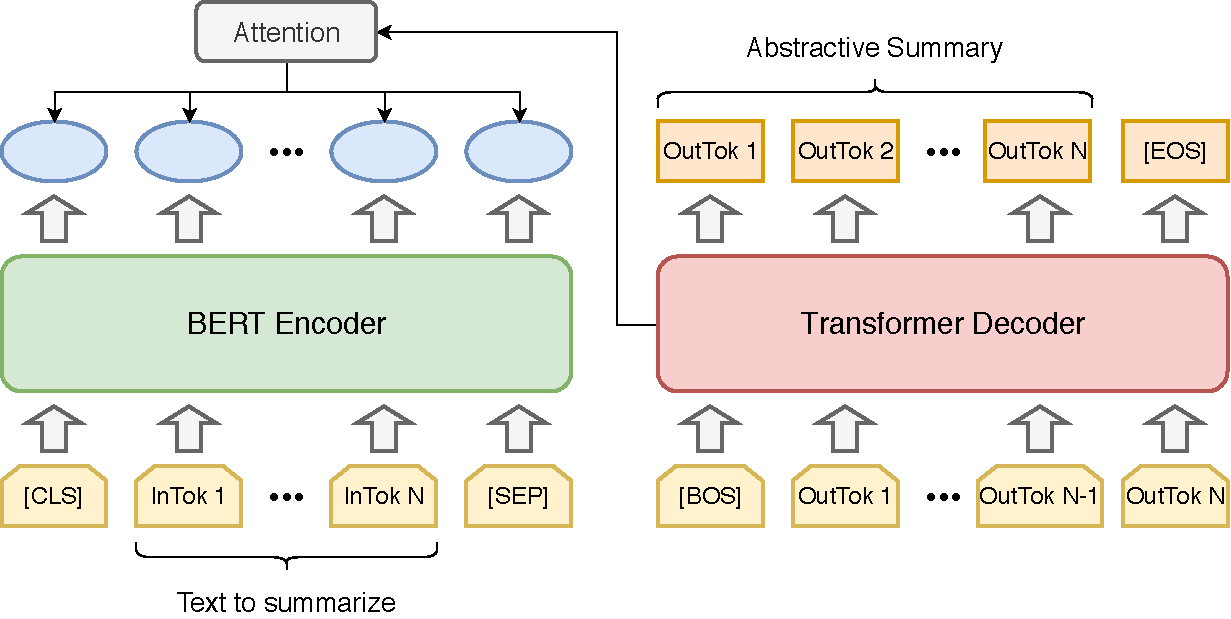
\includegraphics[width=0.7\paperwidth]{figures/summarization-architecture}
\caption{Visualization of the model architecture.}
\label{fig:summarization-architecture}
\end{figure}

The architecture of the model used in this work is pretty simple.
For the encoding part, BERT is used and for decoding, a normal Transformer decoder is used.
Like proposed in \cite{1608.05859}, the input embeddings are tied to the output layer.

As described in \cref{sec:bert}, BERT allows either one or two sentence\footnote{Remember, that sentence is not referring to an actual linguistic sentence} inputs.
For this work, only one sentence is used, as there is no need (and logical way) to split the input into two parts.
The Transformer decoder performs attentions over the full output representations of the encoder.
The full architecture is shown in \cref{fig:summarization-architecture}.

% =======
% TRAINING
% =======

\section{Training}\label{sec:system-description-training}

% TODO I'm pretty sure that there are better examples, but for now this is fine
\begin{figure}[h]
\begin{lstlisting}[numbers=none]
DA1: Thank you very much indeed,
DA2: Cool, thank you,
DA3: So I call the meeting closed.

SUM: They close the meeting by thanking one another.
\end{lstlisting}
\caption{Three dialogue acts (DA1-3) that are linked to one sentence of the summary (SUM).}
\label{fig:dialogue-arc-summary-link-example}
\end{figure}

To circumvent the high memory usage of BERT at long sequence lengths, not the whole meeting transcript is used as input for the network at once.
As described in \cref{sec:ami-meeting-corpus}, for every sentence in a meeting's abstractive summary, there exists a link to one or more dialogue acts.
These are the dialogue act, that influence the content of the sentence the most.
An example for such a link is shown in \cref{fig:dialogue-arc-summary-link-example}.
For training, all of these dialogue acts, that belong to the same summary sentence, are concatenated and then used as the source for the summary.
The summary sentence itself is used as the target summary.

\subsection{Preparation of Training Data}

This subsection desrcribes how the training data is processed.

\paragraph{Format of the Corpus Data}

The corpus data for both the AMI Meeting Corpus and the ICSI Meeting Corpus is available in the NITE XML Toolkit (NXT) format \cite{Carletta2003}.
For automatic parsing, a Java library is available, that makes it possible to write a Java program that traversed through the data and collects the necessary data.
For this work, such a program was developed.
It parses the data from the corpora and creates three tab-sepreated-values (.tsv) files, one for each dataset (training, development, test).

\paragraph{Data Cleaning}

In the AMI and ICSI Meeting Corpus, the transcriptions try to include every spoken word.
This includes speech disfluencies like "hmm", "huh", etc.
As these word do not any meaningful value to a sentence, they are filtered out while processing the data.
Word like "yeah", "nope" or "nah" are kept, because they carry meaning, like agreement or disagreement. 

\paragraph{Data Split}

For the AMI Meeting Corpus, the proposed segmentation described in \cref{ssec:ami-segmentation-of-the-corpus} is used.
As the ISCI Meeting Corpus has no recommended segmentation (see \cref{ssec:icsi-segmentation-of-the-corpus}), always the whole dataset is used, but only to perform cross-corpus validation.

% ===================
% IMPLEMENTATION WITH TEXAR
% ===================

\section{Implementation with Texar}

\begin{lstlisting}[numbers=none,language=Python,caption={Hyperparameters for Transformer decoder},captionpos=b,label=lst:hyperparameters-decoder]
hidden_dim = 768

decoder = {
    'dim': hidden_dim,
    'num_blocks': 6,
    'multihead_attention': {
        'num_heads': 8,
        'output_dim': hidden_dim
    },
    'initializer': {
        'type': 'variance_scaling_initializer',
        'kwargs': {
            'scale': 1.0,
            'mode': 'fan_avg',
            'distribution': 'uniform',
        },
    },
    'poswise_feedforward': 
        tx.modules.default_transformer_poswise_net_hparams(
            output_dim=hidden_dim)
}
\end{lstlisting}

For the actual implementation of the network, the Texar toolkit \cite{hu2019texar} is used.
Texar is an open-source modular toolkit, that provides plenty of useful abstractions for fast prototyping of neural network architectures, with a special focus on natural language processing.
It comes in two nearly identical versions, one for TensorFlow \cite{tensorflow2015-whitepaper} and one for PyTorch \cite{NEURIPS2019_9015}.  
For this work, the TensorFlow version is used.
Texar comes with modules for both BERT as well as regular Transformers and allows for an easy connection of BERT and a Transformer decoder.
The code for the complete architecture is only a few hundred lines of code.
Nearly every hyperparameter like the amount of decoder layers, number of attention head or just simple settings like the learning rate can easily be modified.
As an example, the hyperparamater config for the Transformer decoder is shown in \cref{lst:hyperparameters-decoder}.

% ====================
% EXPLORING HYPERPARAMETERS
% ====================

\section{Exploring Hyperparemeters}

The following section will explore the used hyperparameters.
The parameters were determined empirically by testing multiple variations.
After multiple tests, the following hyperparameters have shown the best results.

\begin{figure}[h]
\centering
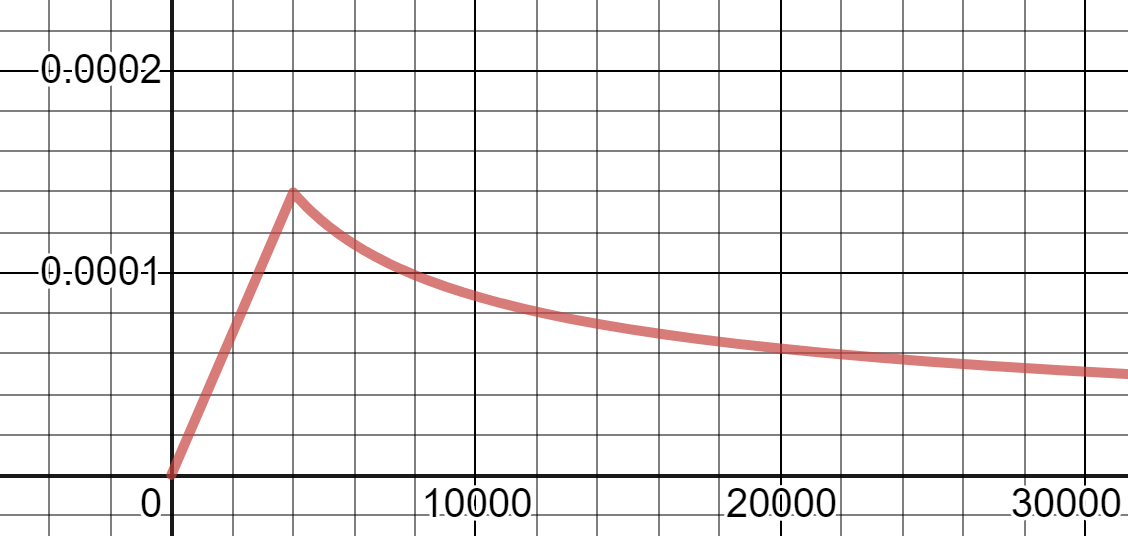
\includegraphics[width=0.6\paperwidth]{figures/learning-rate}
\caption{Visualization of the learning rate with $warmup\_steps = 4000$.}
\label{fig:learning-rate}
\end{figure}

\paragraph{Optimizer and Learning Rate}

The Adam optimizer \cite{article} is used with $\beta_1=0.9$, $\beta_2=0.997$ and $\epsilon = 10^{-9}$.
The learning rate is computed by the following formula:
\[
	learning\_rate = 0.2 \cdot d_{model}^{-0.5} \cdot min(step\_num^{-0.5}, step\_num \cdot warmup\_steps^{-1.5})
\]
which is equivalent to the learning rate used to train the original Transformer \cite[p.~7]{1706.03762}, but multiplied by $0.2$ as this yields better results for this training data as shown be empirical testing.
The warmup steps were set to $warmup\_steps = 4000$.
The formal can be interpreted as linearly increasing the learning rate until $warmup\_steps < steps$ and then steadily decreasing it again.
The function's graph is visualized in \cref{fig:learning-rate}.

\paragraph{Batch-Size and Max-Seq-Length}

Due to memory constraints\footnote{Training was performed on a single Nvidia RTX 2080TI GPU with 11 GB of memory}, it was necessary to find a good balance between the batch size and maximum input sequence length.
For the experiments performed in this thesis, the following values proofed to be a good compromise:
\begin{itemize}
\item A maximum input sequence length of $96$
\item A batch size of $28$
\end{itemize}

Smaller batch sizes harm the networks performance and smaller maximum sequence lengths mean lost information, as some of the inputs are quite long and would be truncated.

\paragraph{Transformer decoder}

For the Transformer decoder, $N=6$ stacked decoder layers are used.
The number of attention heads is set to $8$ and the hidden dimension has a size of $768$, as this the one used by BERT\textsubscript{BASE} model \cite[p.~3]{devlin2018bert}.